\documentclass[border=4pt]{standalone}
\usepackage{tikz}
\usetikzlibrary{arrows.meta,positioning}
\begin{document}
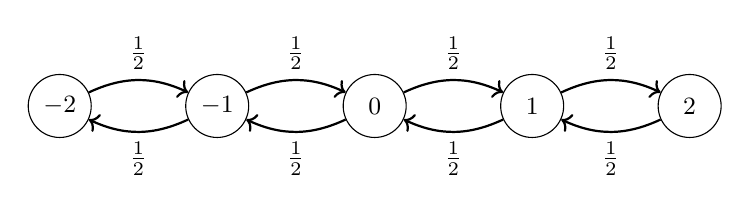
\begin{tikzpicture}[
  node distance=2cm,
  state/.style={circle, draw, minimum size=0.8cm, font=\small}
]
  \node[state] (A) {$-2$};
  \node[state] (B) [right of=A] {$-1$};
  \node[state] (C) [right of=B] {$0$};
  \node[state] (D) [right of=C] {$1$};
  \node[state] (E) [right of=D] {$2$};
  \foreach \from/\to in {A/B, B/C, C/D, D/E} {
    \draw[->, bend left=25, thick] (\from) to node[above] {$\frac{1}{2}$} (\to);
    \draw[->, bend left=25, thick] (\to)   to node[below] {$\frac{1}{2}$} (\from);
  }
\end{tikzpicture}
\end{document}
